\documentclass{standalone}
\usepackage{tikz,tikz-3dplot}
\tikzset{thin_line/.style={very thick, solid, color=black}}
\tikzset{dash_line/.style={thin, dashed, color=darkgray}}
\tikzset{vect_line/.style={very thick, ->, >=latex,  solid, color=black}}
\begin{document}
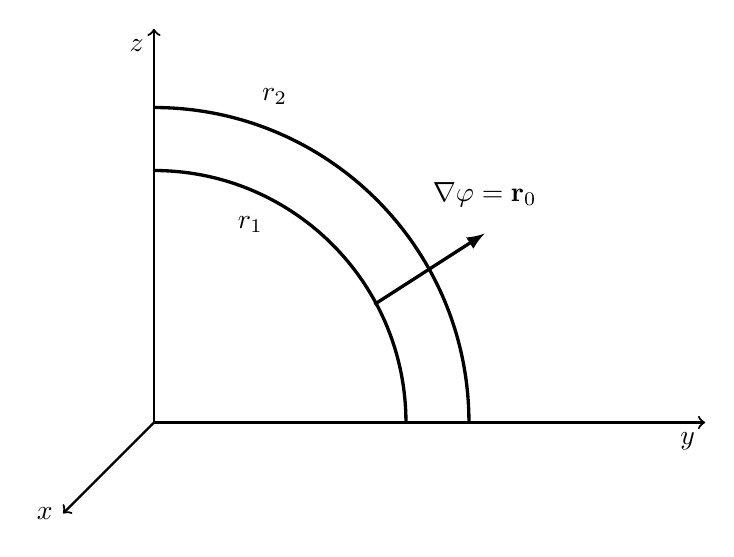
\begin{tikzpicture}[scale=2]
	\draw[thick,->] (-1.5,0,0) -- (2,0,0) node[anchor=north east]{$y$};
	\draw[thick,->] (-1.5,0,0) -- (-1.5,2.5,0) node[anchor=north east]{$z$};
	\draw[thick,->] (-1.5,0,0) -- (-1.5,0,1.5) node[anchor=east]{$x$};
	
	\draw [thin_line] (0.1,0) arc(0:90:1.6) node [below=0.2cm, near end] {$r_{1}$};
	\draw [thin_line] (0.5,0) arc(0:90:2)   node [above=0.2cm, near end] {$r_{2}$};
	
	\draw [vect_line] (-0.1,0.75) -- (0.6,1.2) node[above=0.2cm] {$\nabla \varphi = \mathbf{r}_{0}$};

\end{tikzpicture}
\end{document}